\documentclass[11pt,letterpaper]{article}
\usepackage[lmargin=1in,rmargin=1in,tmargin=1in,bmargin=1in]{geometry}
\usepackage{../style/homework}
\usepackage{../style/commands}
\setbool{quotetype}{true} % True: Side; False: Under
\setbool{hideans}{false} % Student: True; Instructor: False

% -------------------
% Content
% -------------------
\begin{document}

\homework{8: Due 10/27}{Cleanliness becomes more important when godliness is unlikely.}{P.J. O'Rourke}

% Problem 1
\problem{10} Plot the quadratic function $y= 2x^2 - 3x + 4$ as accurately as possible. Your sketch should include the vertex and axis of symmetry. 
	\[
	\fbox{
	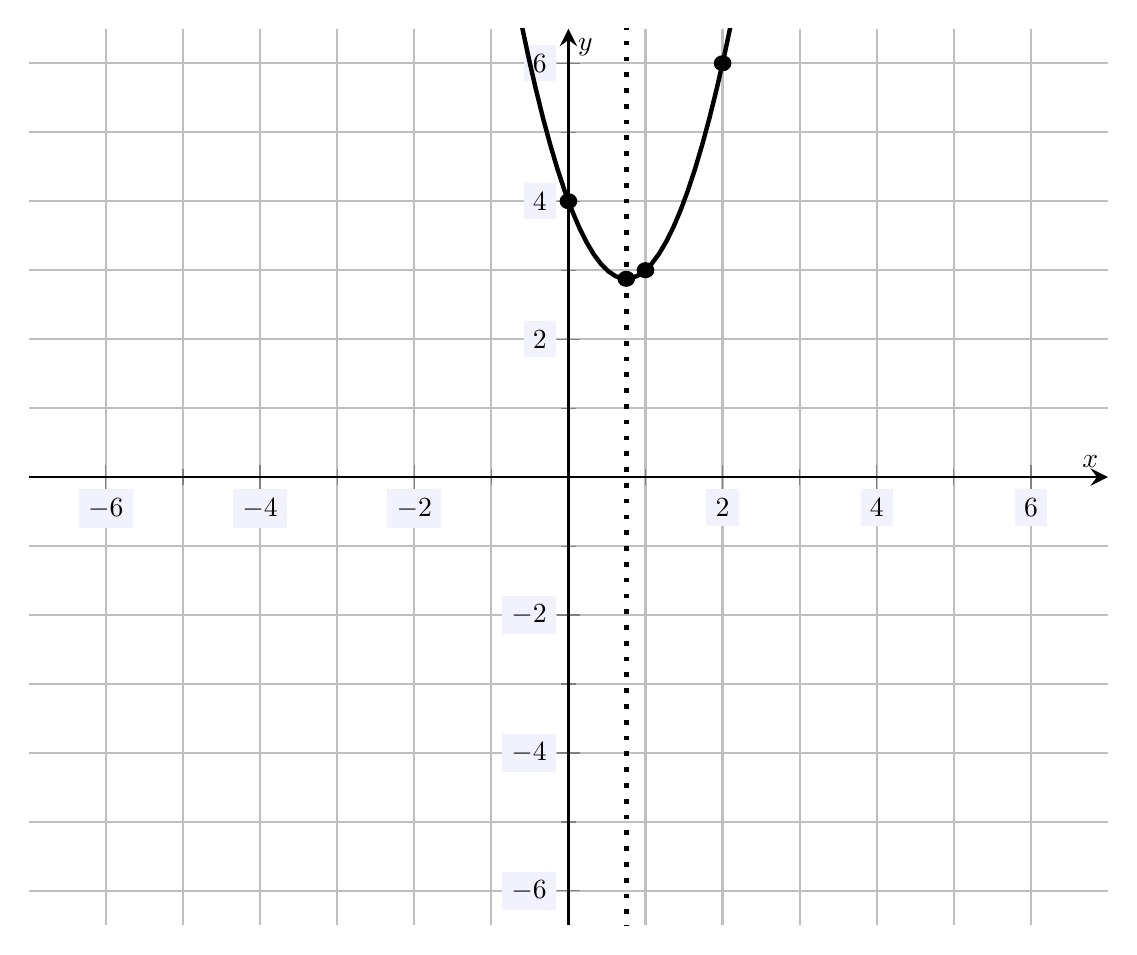
\begin{tikzpicture}[scale=2,every node/.style={scale=0.5}]
	\begin{axis}[
	grid=both,
	axis lines=middle,
	ticklabel style={fill=blue!5!white},
	xmin= -7, xmax=7,
	ymin= -6.5, ymax=6.5,
	xtick={-6,-4,-2,0,2,4,6},
	ytick={-6,-4,-2,0,2,4,6},
	minor tick = {-5,-3,...,5},
	xlabel=\(x\),ylabel=\(y\),
	]
	\addplot[thick, domain= -7:7,samples=150] {2*x^2 - 3*x + 4};
	\draw[dotted,line width= 0.03cm] (3/4,-10) -- (3/4,10);
	\draw[fill=black] (0,4) circle (0.1);
	\draw[fill=black] (3/4,23/8) circle (0.1);
	\draw[fill=black] (1,3) circle (0.1);
	\draw[fill=black] (2,6) circle (0.1);
	\end{axis}
	\end{tikzpicture}
	}
	\] \pspace

Because $a= 2 > 0$, the parabola opens upwards, i.e. is convex. The vertex occurs at $x= -\frac{b}{2a}= -\frac{-3}{2(2)}= \frac{3}{4}$. We know 
	\[
	y(3/4)= 2 \left( \frac{3}{4} \right)^2 - 3 \left( \frac{3}{4} \right) + 4= 2 \cdot \frac{9}{16} - \frac{9}{4} + 4= \frac{9}{8} - \frac{9}{4} + 4= \frac{9}{8} - \frac{18}{8} + \frac{32}{4}= \frac{9 - 18 + 32}{4}= \frac{23}{8}
	\]
Therefore, the vertex is $(3/4, 23/8)$. We need to include this point. The axis of symmetry is $x= \frac{3}{4}$. We find serval other points:
	\begin{table}[!ht]
	\centering
	\begin{tabular}{r||rrrrrrrrrr}
	$x$ & $-4$ & $-3$ & $-2$ & $-1$ & $0$ & $\frac{3}{4}$ & $1$ & $2$ & $3$ & $4$ \\ \hline
	$f(x)$ & $48$ & $31$ & $18$ & $9$ & $4$ & $\frac{23}{8}$ & $3$ & $6$ & $13$ & $24$
	\end{tabular}
	\end{table}





\newpage





% Problem 2
\problem{10} Plot the quadratic function $y= -x^2 - 4x + 1$ as accurately as possible. Your sketch should include the vertex and axis of symmetry. 
	\[
	\fbox{
	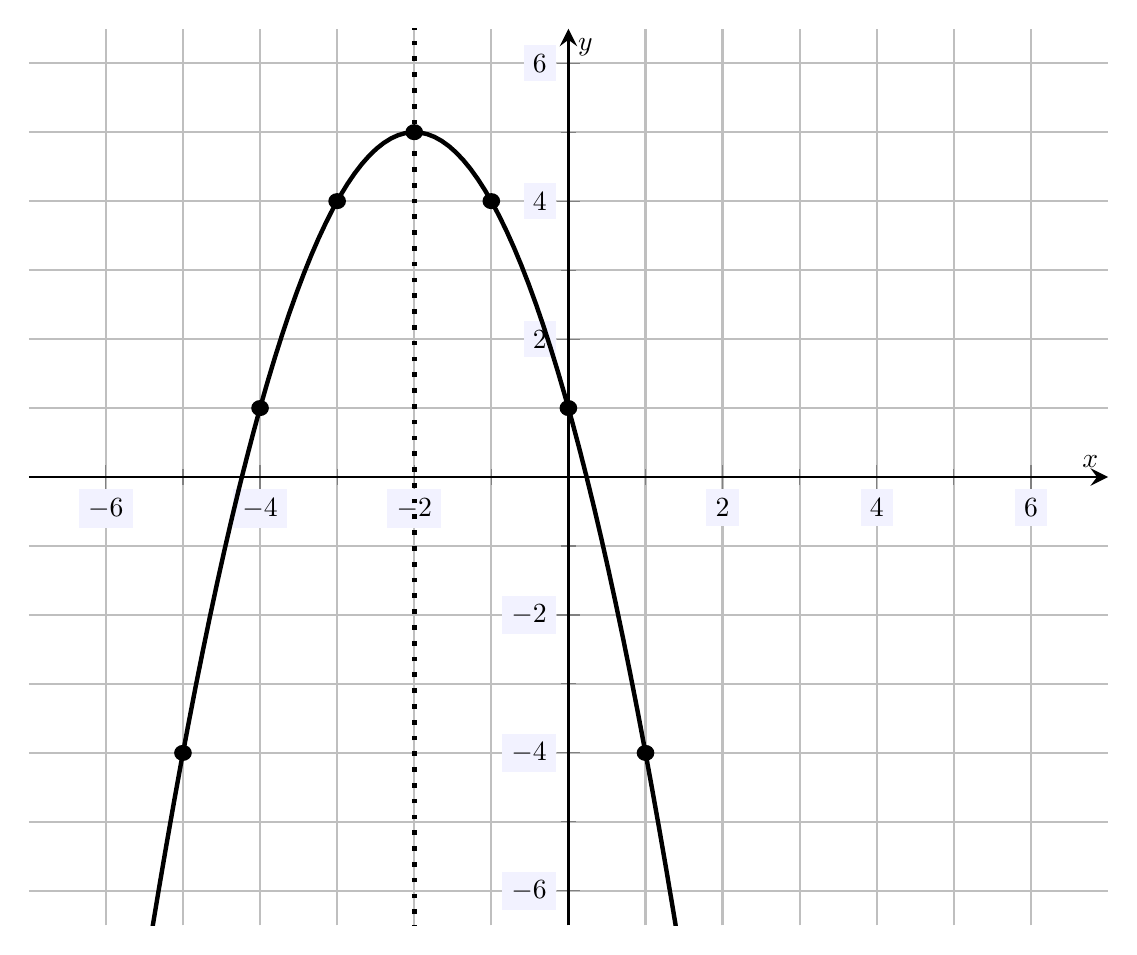
\begin{tikzpicture}[scale=2,every node/.style={scale=0.5}]
	\begin{axis}[
	grid=both,
	axis lines=middle,
	ticklabel style={fill=blue!5!white},
	xmin= -7, xmax=7,
	ymin= -6.5, ymax=6.5,
	xtick={-6,-4,-2,0,2,4,6},
	ytick={-6,-4,-2,0,2,4,6},
	minor tick = {-5,-3,...,5},
	xlabel=\(x\),ylabel=\(y\),
	]
	\addplot[thick, domain= -7:7,samples=150] {-1*x^2 - 4*x + 1};
	\draw[dotted,line width= 0.03cm] (-2,-10) -- (-2,10);
	\draw[fill=black] (-6,-11) circle (0.1);
	\draw[fill=black] (-5,-4) circle (0.1);
	\draw[fill=black] (-4,1) circle (0.1);
	\draw[fill=black] (-3,4) circle (0.1);
	\draw[fill=black] (-2,5) circle (0.1);
	\draw[fill=black] (-1,4) circle (0.1);
	\draw[fill=black] (0,1) circle (0.1);
	\draw[fill=black] (1,-4) circle (0.1);
	\end{axis}
	\end{tikzpicture}
	}
	\] \pspace

Because $a= -1 < 0$, the parabola opens downwards, i.e. is concave. The vertex occurs at $x= -\frac{b}{2a}= -\frac{-4}{2(-1)}= -2$. We know 
	\[
	y(-2)= -(-2)^2 - 4(-2) + 1= -4 + 8 + 1= 5
	\]
Therefore, the vertex is $(-2, 5)$. We need to include this point. The axis of symmetry is $x= -2$. We find serval other points:
	\begin{table}[!ht]
	\centering
	\begin{tabular}{r||rrrrrrrrrrr}
	$x$ & $-6$ & $-5$ & $-4$ & $-3$ & $-2$ & $-1$ & $0$ & $1$ & $2$ & $3$ & $4$ \\ \hline
	$f(x)$ & $-11$ & $-4$ & $1$ & $4$ & $5$ & $4$ & $1$ & $-4$ & $-11$ & $-20$ & $-31$
	\end{tabular}
	\end{table}





\newpage





% Problem 3
\problem{10} Give a rough sketch of the quadratic function $y= 2(x + 1)^2 - 2$. Your sketch should include the vertex and axis of symmetry. 
	\[
	\fbox{
	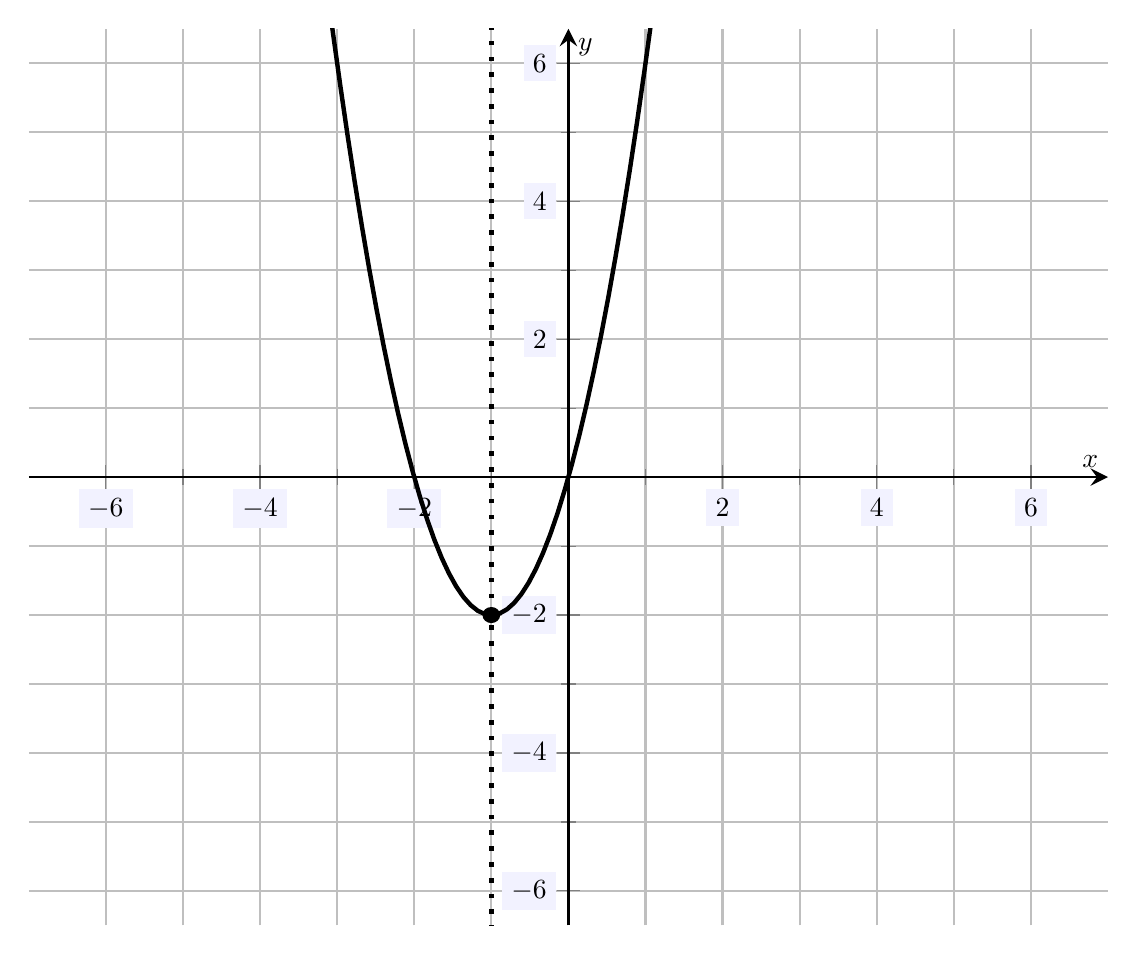
\begin{tikzpicture}[scale=2,every node/.style={scale=0.5}]
	\begin{axis}[
	grid=both,
	axis lines=middle,
	ticklabel style={fill=blue!5!white},
	xmin= -7, xmax=7,
	ymin= -6.5, ymax=6.5,
	xtick={-6,-4,-2,0,2,4,6},
	ytick={-6,-4,-2,0,2,4,6},
	minor tick = {-5,-3,...,5},
	xlabel=\(x\),ylabel=\(y\),
	]
	\addplot[thick, domain= -7:7,samples=150] {2*(x + 1)^2 - 2};
	\draw[dotted,line width= 0.03cm] (-1,-10) -- (-1,10);
	\draw[fill=black] (-1,-2) circle (0.1);
	\end{axis}
	\end{tikzpicture}
	}
	\] \pspace

Because $a= 2 > 0$, the parabola opens upwards, i.e. is convex. Because the parabola is in vertex form, we know the vertex is $(-1, -2)$. Therefore, the axis of symmetry is $x= -1$. 





\newpage





% Problem 4
\problem{10} Give a rough sketch of the quadratic function $y= 5 - (x - 1)^2$. Your sketch should include the vertex and axis of symmetry.  
	\[
	\fbox{
	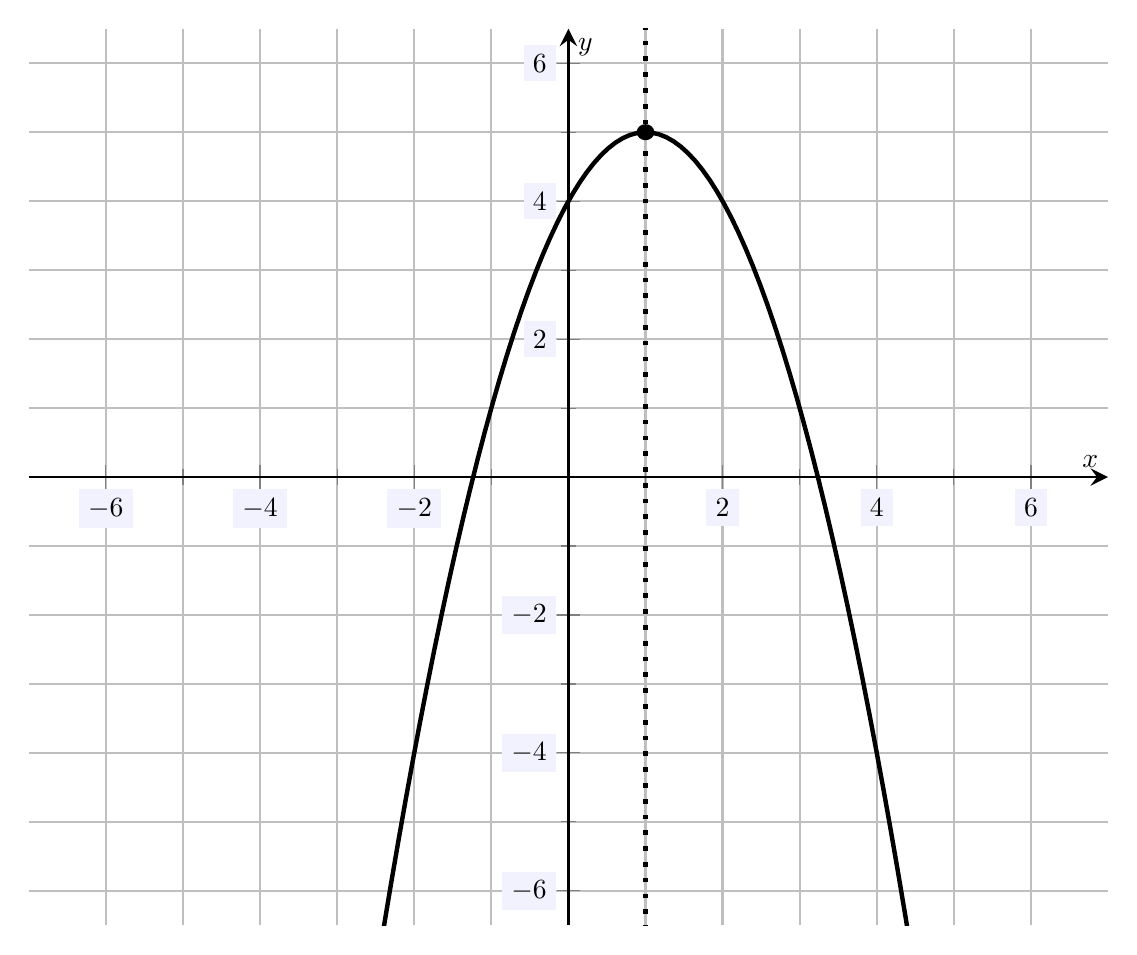
\begin{tikzpicture}[scale=2,every node/.style={scale=0.5}]
	\begin{axis}[
	grid=both,
	axis lines=middle,
	ticklabel style={fill=blue!5!white},
	xmin= -7, xmax=7,
	ymin= -6.5, ymax=6.5,
	xtick={-6,-4,-2,0,2,4,6},
	ytick={-6,-4,-2,0,2,4,6},
	minor tick = {-5,-3,...,5},
	xlabel=\(x\),ylabel=\(y\),
	]
	\addplot[thick, domain= -7:7,samples=150] {5 - (x - 1)^2};
	\draw[dotted,line width= 0.03cm] (1,-10) -- (1,10);
	\draw[fill=black] (1,5) circle (0.1);
	\end{axis}
	\end{tikzpicture}
	}
	\] \pspace

Because $a= -1 < 0$, the parabola opens downwards, i.e. is concave. Because the parabola is in vertex form, we know the vertex is $(1, 5)$. Therefore, the axis of symmetry is $x= 1$. 


%\printpoints
\end{document}